%for DU ASE

\documentclass[12pt]{arsubmit}
\usepackage{graphicx}             %% jpg, gif, tiff, and pdf graphics
\usepackage{moreverb}             %% Verbatim Code Listings
\usepackage{array}
\usepackage{subfigure}
\usepackage{alltt}
\usepackage{algorithm}
\usepackage{algpseudocode}

\begin{document}




\title{NECAMO - New Evolutionary Clustering Algorithm using Multiobjective Optimization}
%\author{Md. Shiplu Hawlader\,$^{1}$\footnote{to whom correspondence should be addressed}$\  $ and Saifuddin Md. Tareeq\,$^{1}$}
\author{Md. Shiplu Hawlader\,$^{1}$, Kaynat Quayyum\,$^{1}$ and Saifuddin Md. Tareeq\,$^{1}$\footnote{to whom correspondence should be addressed}$\  $}
\date{ \center{$^{1}$Department of Computer Science and Engineering \\ University of Dhaka, Dhaka 1000, Bangladesh\\ \it{shiplu.cse.du@gmail.com} , \it{smtareeq@cse.univdhaka.edu}}}

\maketitle
\begin{abstract}
Evolutionary clustering in dynamic networks is the process of generating a sequence of clusters to capture the true nature of evolution in interactions among individuals. There are several different approaches to solve the evolutionary clustering problem and a relatively new one is the multiobjective optimization using genetic algorithms. In this paper, we have proposed a new evolutionary clustering algorithm using multiobjective optimization or NECAMO. Experimental results on real and synthetic data show that the proposed algorithm provides better accuracy compared to previous algorithms in terms of the two relevant parameters - accuracy of clustering with respect to current data and drift from the clusters found from previous steps.
\newline
\newline
\em{Keywords:} Genetic Algorithms, Multiobjective Optimization, Data Mining, Clustering, Dynamic Networks.
\end{abstract}



\section{Introduction}
Individuals or objects are logically connected in networks, either densely, or sparsely. The dense group can be defined as a cluster or community. Clustering is the organization of data patterns into groups based on some measures of similarities or logical connections \cite{jain}. The study of real world dynamic networks is a growing scientific field that combines traditional social network analysis (SNA), link analysis (LA) and multi-agent systems (MAS) within network science and network theory. 
Most of the complex dynamic networks can be modeled as graphs, where nodes represent individual objects and edges represent relation among those individuals. The dynamic behavior of the network can be imposed by keeping a set of graphs for a particular time window. Each static graph in the set corresponds to the network for a particular timestamp. The proximity between individuals can be modeled by putting weight in the edges. The uncertainty however can be established in the transformation of graphs over times. Dynamic network analysis leads to finding pattern in the clustering of a community. Hence, this type of analysis can be beneficial for numerous entities like social network developers, telecommunication operators or for detecting the group of individuals responsible for spamming or junk emails.


Many approaches have been proposed for the analysis and temporal evolution of dynamic networks in \cite{dynmoga1}, \cite{dynmoga3}, \cite{dynmoga12}, \cite{dynmoga13}, \cite{dynmoga14}, \cite{dynmoga15}, \cite{dynmoga21}, \cite{dynmoga23}, \cite{dynmoga24}, \cite{dynmoga25}, \cite{dynmoga26}. To catch the evolution of clusters in dynamic network with temporal data, some of these methods \cite{dynmoga3}, \cite{dynmoga12}, \cite{dynmoga15}, \cite{dynmoga24} employ the concept of Chakrabarti \emph{et. al.} in \cite{chakrabarti}. These methods produce a sequence of clusters by introducing a framework called temporal smoothness. This framework assumes that abrupt changes of clustering in a short time period are not desirable, thus it smooth each community over time. Smoothness is defined by trading-off between two competing criteria. \emph{Snapshot cost}, which means that the clustering should reflect as nearly as possible the current time steps coming data.  And \emph{temporal cost}, which means that each clustering should not change dramatically from the previous time steps.

In this paper we have proposed NECAMO algorithm which implements similar concept as \cite{spea2}, but with an improved fitness assignment scheme. The proposed algorithm performs better in terms of accuracy with respect to previous algorithms. The result is supported by experimentation with synthetic and real data. In the following sections we will elaborate the proposed algorithm.

\section{Related Work}

Several genetic algorithms provided efficient solutions for multiobjective optimizations. Some well-known multiobjective genetic algorithms are vector evaluated GA \cite{vega}, Niched Pareto Genetic Algorithm \cite{npga}, Weight Based Genetic Algorithm \cite{wbga}, Non-dominated Sorting Genetic Algorithm (NSGA)\cite{nsga}, Strength Pareto Evolutionary Algorithm (SPEA) \cite{spea} and more. General problems with all these multi-objective evolutionary algorithms are that computational complexity is $O(MN^3)$ (where M is the number of objectives and N is the population size), their non-elitism approach and the need to specify a sharing parameter.

In Folino et al. \cite{dynmoga} used NSGA2 \cite{nsga2} for detecting communities in dynamic networks. NSGA2 is the improved version of NSGA \cite{nsga} which alleviates all the above three problems by introducing a new selection operator which creates a mating pool by combining the parent and offspring populations and used crowding distance for diversity preservation.
 
In our proposed algorithm, we have used SPEA2 \cite{spea2}. SPEA2 is an improved algorithm of SPEA with respect to fitness and diversity measurement. SPEA2 used an improved fitness assignment scheme, which takes into account how many individuals dominate and dominated by a single individual. SPEA2 used  $k$-th nearest neighbor to preserve diversity of solutions and gives better quality population in short period of time than NSGA2. We have used SPEA2 to predict different cluster of network in different time stamp. In next sections we will show, our proposed algorithm gives better result with respect to \cite{dynmoga}.


\section{Problem Formulation}


Let  $\{1,\ldots,T\}$ be a finite set of time steps and $V = \{1,\ldots,|V|\}$ be a set of individuals or objects. A static network $\mathcal{N}^t$ at time $t$ can be modeled as a graph $G^t = (V^t,E^t)$ where $V^t$ is a set of objects, called nodes or vertices and $E^t$ is a set of links, called edges, that connect two elements of $V^t$ at time $t$. Thus $G^t$ is the graph representing a snapshot of the network $\mathcal{N}^t$ at time $t$. An edge $(u^t, v^t)\in E^t$ if individual $u$ and $v$ have interacted at time $t$.

A dynamic network $\mathcal{N}$ is a sequence of static networks $\{\mathcal{N}^1,\ldots,\mathcal{N}^T\}$, where each network $\mathcal{N}^t$ is a snapshot of the network at timestamp $t$. A cluster in a static network $\mathcal{N}^t$ is a group of vertices consisting of a subset of $V^t$ having a high density of edges inside the cluster and a lower density of edges outside of the cluster \cite{dynmoga}. Let $C^t$ is a sub-graph of $G^t$ be a cluster at time $t$. A clustering $\mathcal{CR}^t = \{C_1^t,\ldots,C_k^t\}$ of network $\mathcal{N}^t$ at time $t$ is a partitioning of the graph $G^t$ in groups of nodes such that for each couple of groups or communities $C_i^t$ and $C_j^t \in  \mathcal{CR}^t$ and $V_i^t \cap V_j^t = \emptyset$.

A multiobjective optimization problem deals with more than one objective functions that are to be minimized or maximized. These objectives can be conflicting, subject to certain constraints and often lead to choosing the best trade-off among them. Evolutionary clustering comprises of two conflicting objective functions to optimize.

\subsection{Multiobjective Evolutionary Clustering}

A multiobjective evolutionary clustering problem $(\Omega,\mathcal{F}_1,\mathcal{F}_2,\ldots,\mathcal{F}_h)$ for a static network $\mathcal{N}^t$ can be defined as $min \mathcal{F}_i(\mathcal{CR}^t)$, $i = 1,\ldots,h$ where $\Omega = \{\mathcal{CR}_1^t,\ldots,\mathcal{CR}_k^t\}$ is the set of feasible clusters of $\mathcal{N}^t$ at time stamp $t$, and $\mathcal{F} = {\mathcal{F}_1,\ldots,\mathcal{F}_h}$ is a set of $h$ single criterion functions \cite{dynmoga}. Each $\mathcal{F}_i\colon \Omega \rightarrow R$ is a different objective function that determines the feasibility of the clustering obtained. $\mathcal{F}$ is a vector of conflicting objectives that must be simultaneously optimized, there is not one unique solution to the problem, but a set of solutions are found through the use of Pareto optimality theory \cite{dynmoga9}. 

Given two solution $\mathcal{CR}_1$ and $\mathcal{CR}_2 \in \Omega$, solution $\mathcal{CR}_1$ is said to dominate solution $\mathcal{CR}_2$, denoted as $\mathcal{CR}_1 \prec \mathcal{CR}_2$, if and only if , \[\forall i \colon \mathcal{F}_i(\mathcal{CR}_1) \leq \mathcal{F}_i(\mathcal{CR}_2) \wedge \exists i\hspace {2 mm} \mathcal{F}_i(\mathcal{CR}_1)<\mathcal{F}_i(\mathcal{CR}_2)\]

That is, all the objective function of $\mathcal{CR}_1$ should be better or equal to $\mathcal{CR}_2$ and at least one objective function is better than $\mathcal{CR}_2$. On the other hand, non-dominated solutions is one for which an upgrading in one objective need a ruin of another. These solutions are called Pareto-optimal. Formally the set of Pareto-optimal solutions $\Pi$ is defined as \[\Pi = \{ \mathcal{CR} \in \Omega \colon \hspace {1 mm} \forall \mathcal{CR}' \in \Omega \hspace {1 mm}with \hspace {1 mm}\mathcal{CR}' \prec \mathcal{CR}\}\]



\subsubsection{ Snapshot cost} 
Snapshot Cost $(SC)$ measures how well a cluster $C^t$ represents the network $\mathcal{N}^t$ at time $t$.  \emph{Community Score} is very effective to detect snapshot cost of cluster \cite{dynmoga19}. Let $\mathcal{CR}^t = \{C_1^t,\ldots,C_k^t\}$ be a clustering of a network $\mathcal{N}^t$ of graph $G^t$ at time $t$. The $community\hspace{1 mm} score$ of $\mathcal{CR}^t$ is defined as follows, 
\begin{equation} \mathcal{CS}(\mathcal{CR}^t) = \sum\limits_{i=1}^k score(C_i^t) \label {eq:one}
\end{equation} where 

\begin{equation} 
score(C_i^t) = \frac{\sum\nolimits_{j\in C^t} {({\mu}_j )}^2} {|C^t|} \times \sum\limits_{i,j\in C^t} A_{ij}^t  \label{eq:two} 
\end{equation}

In equation (\ref{eq:two}),second term represents number of edge connecting nodes inside the community $C^t$. The first term computes the square mean of, \begin{equation} {\mu}_i = \frac{1} {|C^t|} \sum\limits_{j\in C^t} A_{ij}^t\label{eq:three}\end{equation} where $A_{ij}^t$ is the adjacency matrix of 1 and 0.
In equation (\ref{eq:two}) and (\ref{eq:three}) ${\mu}_i$ how tightly a node $i$ is connected in the cluster $C^t$ by fraction of edge connection inside $C^t$.
Thus according to equation (\ref{eq:one}), (\ref{eq:two}) and (\ref{eq:three}) the objective function $community \hspace{1 mm} score$ is considering the number of interconnection inside the community and also outside the community.
More the $community\hspace{1 mm}score$, more the cluster represents the current network $\mathcal{N}^t$.\\

\subsubsection{Temporal cost}
The algorithm should maintain the similarity between the current clusters to the previous time steps clusters. Normalized Mutual Information $(NMI)$, well known entropy measure in information theory, can be used to measure temporal cost. Let two clusters  $A = \{A_1,\ldots,A_n\}$ and $B = \{B_1,\ldots,B_m\}$ of a network. let $M$ be the confusion matrix whose cell $M_{ij}$ represents how many nodes in cluster $A_i \in A $ that are also in the cluster $B_j \in B$. The Normalized Mutual Information $(NMI)$ is defined as, 

\begin{equation} NMI(A,B) =\frac{ -2 \sum\limits_{i=1}^n\sum\limits_{j=1}^m M_{ij}\log {\frac {M_{ij}N}{M_{i.}M_{.j}}} }{\sum\limits_{i=1}^nM_{i.}\log{(M_{i.}/N)} + \sum\limits_{j=1}^mM_{.j}\log{(M_{.j}/N)}}\label{eq:four}
\end{equation} 

where $n$ and $m$ are number of groups of the clustering A and B respectively, $M_{i.}$ and $M_{.j}$ are sum of the $i-th$ row and sum of the $j-th$ column of confusion matrix $M$ respectively and N is the number of nodes in the network. $NMI$ is a value between 0 and 1. If clustering $A$ and $B$ are same, that is $A = B$, then $NMI(A,B)=1$ and if A and B are completely different then $NMI(A,B) =0$. Thus the objective function for this problem $NMI(\mathcal{CR}^t,\mathcal{CR}^{t-1})$ are to be maximized.


\subsection{Multiobjective Genetic Algorithm}
Genetic Algorithms $(GA)$ can provide very efficient solutions for multi-objective optimizations. A generic single objective GA can be modified to find a set of multiple non-dominated solutions in clustering method. A multi-objective GA should have a good fitness function, should preserve the diversity and should maintain elitism. 

\section{Proposed Algorithm}
The proposed algorithm takes a dynamic network $\mathcal{N} = \{\mathcal{N}_1, \mathcal{N}_2,\ldots,\mathcal{N}_T\}$, the sequence of graphs $G = \{G_1,G_2,\ldots,G_T\}$ and the number of timestamps $T$ as input and gives a clustering of each network $\mathcal{N}_i$ of $\mathcal{N}$ as output.
\subsection {Initialization}
For the first timestamp of first input network there is no temporal relation with the previous network. The clustering algorithm is applied only in snapshot cost.
\subsection {Population from Graph}
As a first step in each timestamp from 2nd timestamp to $T$, it creates a population of random individuals. Each individual is a vector of length equal to number of nodes in the graph $G^t$. 
\begin{figure}
\centering
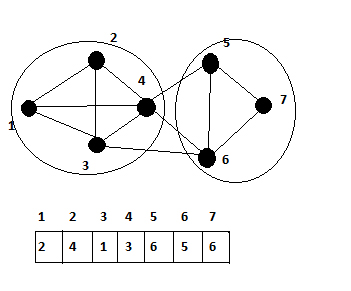
\includegraphics[width=0.5\textwidth]{graph}
\caption {Network of 7 nodes clustered into \{1,2,3,4\} and \{5,6,7\} and their genetic reprsentation}
\label {fig:graph}
\end{figure}
\subsection {Decoding}
As each individual gene is working as an adjacency list, if a node in $u$ of graph is reachable from $v$ by maintaining the edges in the individual, then $u$ and $v$ is in same cluster of component.
\subsection {Evaluation}
In this algorithm the evaluation phase consist of calculating community score, which defines how better is the current clustering with respect to the given network and normalized mutual information ($NMI$), which defines the clustering fluctuation from the previous timestamp. 
\subsection {Assign Rank}
Each individual of the population and archive is given a rank value, the smaller the better. After giving each individuals a rank value, sort the individuals according to the ascending rank. 
\begin {equation}
r(v) = \sum\nolimits_{v\prec u} s(u)
\label {eq:rank}
\end {equation}

\subsection {Fitness Function}
To remain the population diverse, we are using distance of $k-th$ nearest neighbor. The fitness value of each individual is the sum of its non-dominated rank and the inverse of the distance of $k-th$ nearest neighbors distance. 
\begin{equation}
f(v) = r(v)+ {({\sigma}_v^k + 1)}^{-1}
\label{eq:density}
\end{equation}
where ${\sigma}_v^k$ is the distance between individual $v$ and its $k-th$ nearest neighbor.
\subsection {Population Selection}
From the total individuals of population and archive population size individuals are selected as new population. From the rank 0 to the highest rank, all the individuals are added if number of population of this rank is not exceeding the current population size. If it is exceeding, then some individuals are truncated according to the value of each individuals.
\subsection {Mating Pool Creation}
A mating pool is created of pool size from the new population to apply the genetic variation operators. To choose the mating pool, binary tournament with replacement has been used in this algorithm. 
\subsection {Genetic Variation Operators}
Genetic operators are used to create offspring from parent or mating pool. There are two widely used genetic variation operators namely crossover and mutation. In the following subsection a short description of these two operators is given. 

 
\subsubsection {Crossover}
In this algorithm we are using uniform crossover. A random bit vector of length of number of the node in the current graph is created. If $i-th$ bit is 0 then the value of the $i-th$ gene comes from the first parent otherwise it comes from the $i-th$ gene of second parent. As each of the parents holding true adjacency information, the offspring will also hold it.\\
\begin {table}
\begin{center}
\begin {tabular} { p{3 cm} l l l l l l l}
\hline
Parent1: & 4 & 3 & 2 & 2 & 6 & 5 & 6\\
Parent2: & 3 & 3 & 1 & 5 & 4 & 7 & 6\\
Mask : & 0 & 1 & 1 & 0 & 0 & 1 &1\\
Offspring: & 4 & 3 & 1 & 2 & 6 &7 & 6\\
\hline
\end {tabular}
\end{center}
\caption {Example of Uniform Crossover}
\end {table}
\subsubsection {Mutation}
To mutate and create a offspring, some position of the of the individuals are chosen randomly and changed to other values. But the value should be one of its neighbors in the current graph.
\subsection {Archive}
After variation operators over the offspring becomes the new population and the old populations are saved to the archive. To fit the archive size, the truncation mechanism used here also. \\



\begin{algorithm}
\caption{Algorithm: New Clustering Algorithm using Multiobjective Optimization (NECAMO)}
\label{necamo}
\begin{algorithmic}[1]
\Procedure{NECAMO}{$\mathcal{N} = \{\mathcal{N}^1,\ldots,\mathcal{N}^T\}$ a dynamic network of graph $G = \{G^1,\ldots,G^T\}$}

\State Generate initial cluster $\mathcal{CR}_1 = \{C_1^1,\ldots,C_k^1\}$ of thenetwork $\mathcal{N}^1$ by optimizing only $(\mathcal{SC})$
\State let $t = 2$


\While{$t \leq T$}
\State Create initial population of random individual $P_0$ and set $E_0 = \emptyset, i = 0$
\While{$\Delta f(v) \ge 10^{-5}$}
\State Select individuals from $E_i$ for mating pool using binary tournament with replacement
\State Apply crossover and mutation to create $N_P$ offspring solutions. Copy offspring to $P_i$
\State Decode each individual of $P_i \cup E_i$ \label{decode}
\State Evaluate each individual of $P_i \cup E_i$  and assign fitness value  using equation \ref {eq:density}

\State Copy all non-dominated solutions to $E_{i+1}$
\If {$|E_{i+1}| > N_E$}
\State truncate $|E_{i+1}| - N_E$ solutions according to maximum density value
\Else
\State copy best $N_E - |E_{i+1}|$ dominated solutions according to their fitness value
\EndIf
\State  Set $i = i +1$
\EndWhile
\State $C_t = E$ with highest modularity 
\State Set $t = t +1$
\EndWhile
\State Return the clustering set $C$ with best cluster. \label{last}
\EndProcedure
\end{algorithmic}
\end{algorithm}


\section {Performance Analysis}
NMI and modularity are calculated as a measure of performance. Modularity defines the goodness of a clustering. Good clustering, which have high value of modularity, are those in which there are dense internal connections between the nodes within cluster but only sparse connections between different clusters. In this algorithm we use the modularity, introduced by Girvan and Newman \cite{dynmoga16}. Let $k$ be the number of clusters found inside a network, the modularity $Q$ is defined as,
\begin{equation}
Q = \sum\limits_{C=1}^k \left[ \frac {l_C} {m} - {\left(\frac {d_C}{2m}\right)}^2\right]
\end{equation}
where $m$ is the number of edges of the network, $l_C$ is the total number of edges joining vertices inside the cluster $C$, and $d_C$ is the sum of the degrees of the nodes of cluster $C$.

\section {Experimental Result}
In this section we will discuss the experimental result and its effectiveness and compare the result with one of the recent the algorithm namely Dyn-Moga proposed by Folino \emph{et. al.} in \cite{dynmoga}. For this purpose we used synthetic data as well as real life data. In both cases, our proposed algorithm successfully detects network structure and is very competitive with respect to other algorithms.
Some standard parameter for the genetic algorithm are crossover probability 80\%, mutation probability 20\% and binary tournament for pool selection \cite{goldberg}. The population size was 200, archive size of elitism was 200 and number of generations 300.
\subsection {Synthetic Data}

We have created two types of synthetic data, in one number of different cluster in each timestamp is fixed and in other one number of cluster changes with timestamp. 
For the first type of network, we fixed number of node 128 and it is divided into 4 groups each of 32 nodes. Each node has average degree of 16. As in \cite{dynmoga} we have fixed two parameter $Z_{in}$ and $Z_{out}$.  Each node has $Z_{in}$ number of connection to the internal nodes in which cluster it is situated and $Z_{out}$ number of connection to the outside of the cluster. These connections are created randomly. Total ten network data has been created for ten timestamp. 

For the second type of network, we have changed the number of clusters in a timestamp to test whether the algorithm can detect the change in network structure. Total number of node this time is 256 and for the first timestamp it is divided into 4 clusters, each having 64 nodes. Ten consecutive networks are generated by choosing eight nodes from each community and generating new cluster with these 32 nodes. 

\begin{figure}
\centering
{\label {fig:NMI-zout3-fixed}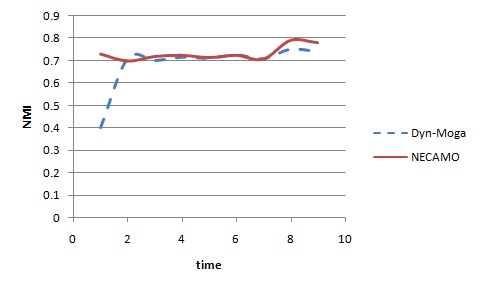
\includegraphics[width=0.5\textwidth]{zout3NMI}}
{\label{fig:NMI-zout5-fixed}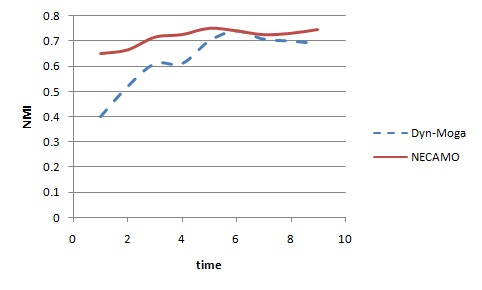
\includegraphics[width=0.5\textwidth]{zout5NMI}}
\caption{Normalized Mutual Information with fixed clustering when $Z_{out} = 3$ (top) and $Z_{out}= 5$ (bottom).}
\label {fig:NMI-fixed}
\end{figure}

\begin{figure}
\centering
{\label {fig:NMI-zout3-var}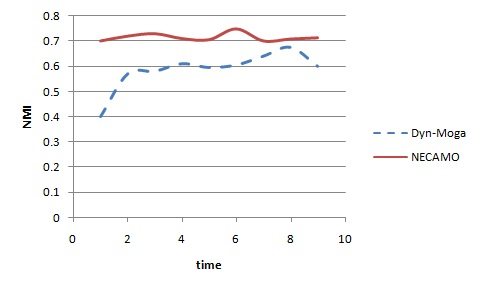
\includegraphics[width=0.5\textwidth]{zout3NMIvar}}
{\label{fig:NMI-zout5-var}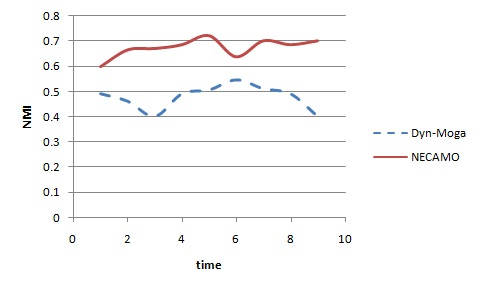
\includegraphics[width=0.5\textwidth]{zout5NMIvar}}
\caption{Normalized Mutual Information with variable clustering when $Z_{out} = 3$ (top) and $Z_{out}= 5$ (bottom).}
\label {fig:NMI-var}
\end{figure}

\begin{figure}
\centering
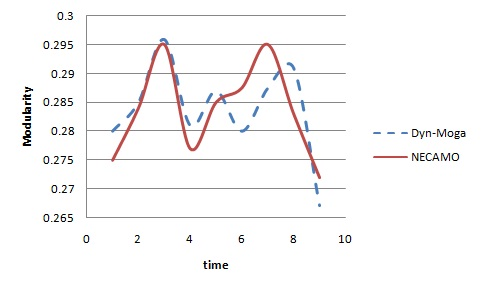
\includegraphics[width=0.5\textwidth]{synth-modul}
\caption {Modularity values obtain with fixed clustering and $Z_{out} = 3$}
\label {fig:synth-modul}
\end{figure}

Figure: \ref{fig:NMI-fixed} shows the obtained result for the synthetic data with fixed number of clustering. In Figure: \ref{fig:NMI-fixed}.1 shows that $NMI$ value with $Z_{out} = 3$ for \cite{dynmoga} and our proposed algorithm are close but in Figure: \ref{fig:NMI-fixed}.2 our algorithm outperforms the \cite{dynmoga} algorithm with $Z_{out} = 5$.
According to Figure: \ref{fig:NMI-var} our algorithm is much stable in historical aspect with respect to \cite{dynmoga}. It also have better modularity in both case of synthetic data compared to \cite{dynmoga} according to Figure: \ref{fig:synth-modul}.

\subsection {Real-life Data}
As real life data set we have chosen the Football data\footnote[1]{http://www.jhowell.net/cf/scores/scoresindex.htm} from the United States college football. The football data is from NCAA Football Division 1-A games. Nodes in the graph represent the team and edges represent the regular season games between two teams they connect. The teams are divided into conferences and they tend to play between members of the same conference. Thus the team cluster is assumed to be the conference. We selected 5 years data from 2006 to 2010 as the 5 timestamps network. Total nodes are 180, 197, 204, 208 and 216 respectively. 
\begin{figure}
\centering
{\label {fig:NMI-real}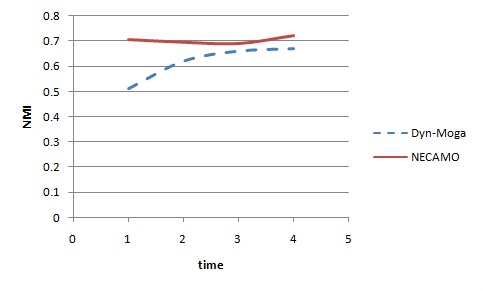
\includegraphics[width=0.5\textwidth]{real-data-NMI}}
{\label{fig:module-real}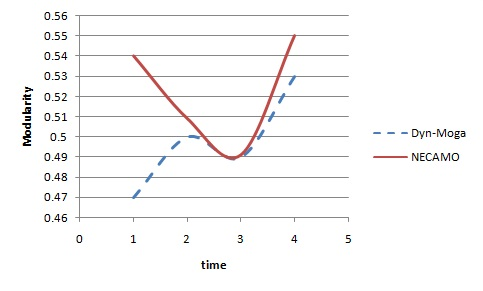
\includegraphics[width=0.5\textwidth]{real-modul}}
\caption{Result obtained with real-life data, NMI and Modularity}
\label {fig:real-data}
\end{figure}
The Figure: \ref{fig:real-data} shows that, our proposed algorithm outperforms the \cite{dynmoga} algorithm in case of normalized mutual information (Figure: \ref{fig:real-data}.1) and Modularity (Figure: \ref{fig:real-data}.2).\\
After these analysis we are claiming that, our proposed algorithm will perform better and give more accurate result  with compared to previous algorithms on evolutionary clustering.

\section {Conclusion}
The need for accuracy and performance in the field of evolutionary algorithm are the reason for our algorithm to implement. In this paper we have provided a multiobjective genetic algorithm.  The algorithm gives best solution which is a trade-off between two objectives current data and displacement from history, at each steps of the algorithm. Experimental results on real and synthetic data show that the proposed algorithm provides better accuracy compared to previous algorithms in terms of the two relevant parameters - accuracy of clustering with respect to current data and drift from the clusters found from previous steps. The future work will be to use adjacency list instead of matrix for genetic representation and the nature of our algorithm suggest that the proposed algorithm can be implemented in parallel system and both future work is expected to improve the time complexity.
 
\bibliographystyle{abbrv}
\bibliography{duase}  % sigproc.bib is the name of the Bibliography in this case

\end{document}
